\ifx\wholebook\relax\else

% --------------------------------------------
% Lulu:

    \documentclass[a4paper,12pt,twoside]{../includes/ThesisStyle}

	\usepackage[T1]{fontenc} %%%key to get copy and paste for the code!
%\usepackage[utf8]{inputenc} %%% to support copy and paste with accents for frnehc stuff
\usepackage{times}
\usepackage{ifthen}
\usepackage{xspace}
\usepackage{alltt}
\usepackage{latexsym}
\usepackage{url}            
\usepackage{amssymb}
\usepackage{amsfonts}
\usepackage{amsmath}
\usepackage{stmaryrd}
\usepackage{enumerate}
\usepackage{cite}
%\usepackage[pdftex,colorlinks=true,pdfstartview=FitV,linkcolor=blue,citecolor=blue,urlcolor=blue]{hyperref}
\usepackage{xspace}
%\usepackage{graphicx}
\usepackage{subfigure}
\usepackage[scaled=0.85]{helvet}
        
        
\newcommand{\sepe}{\mbox{>>}}
\newcommand{\pack}[1]{\emph{#1}}
\newcommand{\ozo}{\textsc{oZone}\xspace}
\newcommand\currentissues{\par\smallskip\textbf{Current Issues -- }}

\newboolean{showcomments}
\setboolean{showcomments}{true}
\ifthenelse{\boolean{showcomments}}
  {\newcommand{\bnote}[2]{
	\fbox{\bfseries\sffamily\scriptsize#1}
    {\sf\small$\blacktriangleright$\textit{#2}$\blacktriangleleft$}
    % \marginpar{\fbox{\bfseries\sffamily#1}}
   }
   \newcommand{\cvsversion}{\emph{\scriptsize$-$Id: macros.tex,v 1.1.1.1 2007/02/28 13:43:36 bergel Exp $-$}}
  }
  {\newcommand{\bnote}[2]{}
   \newcommand{\cvsversion}{}
  } 


\newcommand{\here}{\bnote{***}{CONTINUE HERE}}
\newcommand{\nb}[1]{\bnote{NB}{#1}}
\newcommand{\fix}[1]{\bnote{FIX}{#1}}
%%%% add your own macros 

\newcommand{\sd}[1]{\bnote{Stef}{#1}}
\newcommand{\ja}[1]{\bnote{Jannik}{#1}}
\newcommand{\na}[1]{\bnote{Nico}{#1}}
%%% 


\newcommand{\figref}[1]{Figure~\ref{fig:#1}}
\newcommand{\figlabel}[1]{\label{fig:#1}}
\newcommand{\tabref}[1]{Table~\ref{tab:#1}}
\newcommand{\layout}[1]{#1}
\newcommand{\commented}[1]{}
\newcommand{\secref}[1]{Section \ref{sec:#1}}
\newcommand{\seclabel}[1]{\label{sec:#1}}

%\newcommand{\ct}[1]{\textsf{#1}}
\newcommand{\stCode}[1]{\textsf{#1}}
\newcommand{\stMethod}[1]{\textsf{#1}}
\newcommand{\sep}{\texttt{>>}\xspace}
\newcommand{\stAssoc}{\texttt{->}\xspace}

\newcommand{\stBar}{$\mid$}
\newcommand{\stSelector}{$\gg$}
\newcommand{\ret}{\^{}}
\newcommand{\msup}{$>$}
%\newcommand{\ret}{$\uparrow$\xspace}

\newcommand{\myparagraph}[1]{\noindent\textbf{#1.}}
\newcommand{\eg}{\emph{e.g.,}\xspace}
\newcommand{\ie}{\emph{i.e.,}\xspace}
\newcommand{\ct}[1]{{\textsf{#1}}\xspace}


\newenvironment{code}
    {\begin{alltt}\sffamily}
    {\end{alltt}\normalsize}

\newcommand{\defaultScale}{0.55}
\newcommand{\pic}[3]{
   \begin{figure}[h]
   \begin{center}
   \includegraphics[scale=\defaultScale]{#1}
   \caption{#2}
   \label{#3}
   \end{center}
   \end{figure}
}

\newcommand{\twocolumnpic}[3]{
   \begin{figure*}[!ht]
   \begin{center}
   \includegraphics[scale=\defaultScale]{#1}
   \caption{#2}
   \label{#3}
   \end{center}
   \end{figure*}}

\newcommand{\infe}{$<$}
\newcommand{\supe}{$\rightarrow$\xspace}
\newcommand{\di}{$\gg$\xspace}
\newcommand{\adhoc}{\textit{ad-hoc}\xspace}

\usepackage{url}            
\makeatletter
\def\url@leostyle{%
  \@ifundefined{selectfont}{\def\UrlFont{\sf}}{\def\UrlFont{\small\sffamily}}}
\makeatother
% Now actually use the newly defined style.
\urlstyle{leo}



	\usepackage{amsmath,amssymb}             % AMS Math
% \usepackage[french]{babel}
\usepackage[latin1]{inputenc}
\usepackage[T1]{fontenc}
\usepackage[left=1.5in,right=1.3in,top=1.1in,bottom=1.1in,includefoot,includehead,headheight=13.6pt]{geometry}
\renewcommand{\baselinestretch}{1.05}

\usepackage{multicol}

% Table of contents for each chapter

\usepackage[nottoc, notlof, notlot]{tocbibind}
\usepackage{minitoc}
\setcounter{minitocdepth}{1}
\mtcindent=15pt
% Use \minitoc where to put a table of contents

\usepackage{enumitem}

\usepackage{aecompl}

% Glossary / list of abbreviations

%\usepackage[intoc]{nomencl}
%\renewcommand{\nomname}{List of Abbreviations}
%
%\makenomenclature

% My pdf code

\usepackage[pdftex]{graphicx}
\usepackage[a4paper,pagebackref,hyperindex=true]{hyperref}

\usepackage{pgfplotstable,booktabs,colortbl}
\pgfplotsset{compat=1.8}

% Links in pdf
\usepackage{color}
\definecolor{linkcol}{rgb}{0,0,0.4} 
\definecolor{citecol}{rgb}{0.5,0,0} 

% Change this to change the informations included in the pdf file

% See hyperref documentation for information on those parameters

\hypersetup
{
bookmarksopen=true,
pdftitle="Sista: a Metacircular Architecture for Runtime Optimisation Persistence",
pdfauthor="Clement BERA", 
pdfsubject="Thesis", %subject of the document
%pdftoolbar=false, % toolbar hidden
pdfmenubar=true, %menubar shown
pdfhighlight=/O, %effect of clicking on a link
colorlinks=true, %couleurs sur les liens hypertextes
pdfpagemode=None, %aucun mode de page
pdfpagelayout=SinglePage, %ouverture en simple page
pdffitwindow=true, %pages ouvertes entierement dans toute la fenetre
linkcolor=linkcol, %couleur des liens hypertextes internes
citecolor=citecol, %couleur des liens pour les citations
urlcolor=linkcol %couleur des liens pour les url
}

% definitions.
% -------------------

\setcounter{secnumdepth}{3}
\setcounter{tocdepth}{1}

% Some useful commands and shortcut for maths:  partial derivative and stuff

\newcommand{\pd}[2]{\frac{\partial #1}{\partial #2}}
\def\abs{\operatorname{abs}}
\def\argmax{\operatornamewithlimits{arg\,max}}
\def\argmin{\operatornamewithlimits{arg\,min}}
\def\diag{\operatorname{Diag}}
\newcommand{\eqRef}[1]{(\ref{#1})}

\usepackage{rotating}                    % Sideways of figures & tables
%\usepackage{bibunits}
%\usepackage[sectionbib]{chapterbib}          % Cross-reference package (Natural BiB)
%\usepackage{natbib}                  % Put References at the end of each chapter
                                         % Do not put 'sectionbib' option here.
                                         % Sectionbib option in 'natbib' will do.
\usepackage{fancyhdr}                    % Fancy Header and Footer

% \usepackage{txfonts}                     % Public Times New Roman text & math font
  
%%% Fancy Header %%%%%%%%%%%%%%%%%%%%%%%%%%%%%%%%%%%%%%%%%%%%%%%%%%%%%%%%%%%%%%%%%%
% Fancy Header Style Options

\pagestyle{fancy}                       % Sets fancy header and footer
\fancyfoot{}                            % Delete current footer settings

%\renewcommand{\chaptermark}[1]{         % Lower Case Chapter marker style
%  \markboth{\chaptername\ \thechapter.\ #1}}{}} %

%\renewcommand{\sectionmark}[1]{         % Lower case Section marker style
%  \markright{\thesection.\ #1}}         %

\fancyhead[LE,RO]{\bfseries\thepage}    % Page number (boldface) in left on even
% pages and right on odd pages
\fancyhead[RE]{\bfseries\nouppercase{\leftmark}}      % Chapter in the right on even pages
\fancyhead[LO]{\bfseries\nouppercase{\rightmark}}     % Section in the left on odd pages

\let\headruleORIG\headrule
\renewcommand{\headrule}{\color{black} \headruleORIG}
\renewcommand{\headrulewidth}{1.0pt}
\usepackage{colortbl}
\arrayrulecolor{black}

\fancypagestyle{plain}{
  \fancyhead{}
  \fancyfoot{}
  \renewcommand{\headrulewidth}{0pt}
}

\usepackage{algorithm}
\usepackage[noend]{algorithmic}

%%% Clear Header %%%%%%%%%%%%%%%%%%%%%%%%%%%%%%%%%%%%%%%%%%%%%%%%%%%%%%%%%%%%%%%%%%
% Clear Header Style on the Last Empty Odd pages
\makeatletter

\def\cleardoublepage{\clearpage\if@twoside \ifodd\c@page\else%
  \hbox{}%
  \thispagestyle{empty}%              % Empty header styles
  \newpage%
  \if@twocolumn\hbox{}\newpage\fi\fi\fi}

\makeatother
 
%%%%%%%%%%%%%%%%%%%%%%%%%%%%%%%%%%%%%%%%%%%%%%%%%%%%%%%%%%%%%%%%%%%%%%%%%%%%%%% 
% Prints your review date and 'Draft Version' (From Josullvn, CS, CMU)
\newcommand{\reviewtimetoday}[2]{\special{!userdict begin
    /bop-hook{gsave 20 710 translate 45 rotate 0.8 setgray
      /Times-Roman findfont 12 scalefont setfont 0 0   moveto (#1) show
      0 -12 moveto (#2) show grestore}def end}}
% You can turn on or off this option.
% \reviewtimetoday{\today}{Draft Version}
%%%%%%%%%%%%%%%%%%%%%%%%%%%%%%%%%%%%%%%%%%%%%%%%%%%%%%%%%%%%%%%%%%%%%%%%%%%%%%% 

\newenvironment{maxime}[1]
{
\vspace*{0cm}
\hfill
\begin{minipage}{0.5\textwidth}%
%\rule[0.5ex]{\textwidth}{0.1mm}\\%
\hrulefill $\:$ {\bf #1}\\
%\vspace*{-0.25cm}
\it 
}%
{%

\hrulefill
\vspace*{0.5cm}%
\end{minipage}
}

\let\minitocORIG\minitoc
\renewcommand{\minitoc}{\minitocORIG \vspace{1.5em}}

\usepackage{multirow}
\usepackage{slashbox}

\newenvironment{bulletList}%
{ \begin{list}%
	{$\bullet$}%
	{\setlength{\labelwidth}{25pt}%
	 \setlength{\leftmargin}{30pt}%
	 \setlength{\itemsep}{\parsep}}}%
{ \end{list} }

\newtheorem{definition}{D�finition}
\renewcommand{\epsilon}{\varepsilon}

% centered page environment

\newenvironment{vcenterpage}
{\newpage\vspace*{\fill}\thispagestyle{empty}\renewcommand{\headrulewidth}{0pt}}
{\vspace*{\fill}}



	\graphicspath{{.}{../figures/}}
	\begin{document}
\fi

\chapter{Validation}
\label{chap:validation}
\minitoc


To validate the Sista architecture, we evaluated in Section \ref{sec:bench} the execution time of a set of benchmarks on the Pharo VM with and without the Sista architecture. The VM was also evaluated in different configuration to show the overhead of profiling counters and the persistance of optimisations across multiple start-ups. Section \ref{sec:otherValid} discusses other strategies we implemented to validate our architecture.

\section{Benchmarks}
\label{sec:bench}

%TODO use a citation instead of footnote

We evaluate our architecture on a variety of benchmarks from the Squeak/Smalltalk speed center~\cite{Felg16a} that is used to monitor the performance of the Cog VM and other compatible virtual machines for Squeak and Pharo. The benchmarks are adapted from the Computer Language Benchmarks Game suite \cite{GameBenchs} and contributed by the Smalltalk community. We have selected these benchmarks to give an indication of how certain combinations of operations are optimised with our architecture. Although they tend to over-emphasize the effectiveness of certain aspects of a VM, they are widely used by VM authors to give an indication of performance.

We consider the results on the Pharo VM with four different configurations:
\begin{enumerate}
	\item \emph{Cog} is the existing VM (interpreter and Cogit as the baseline JIT). Cog represents the baseline performance.
	\item \emph{Cog+Counters} is the existing VM with profiling counters without any additional optimisation. Cog+Counters is used to evaluate the profiling counters overhead.
	\item \emph{Sista Cold} is the Sista VM started on a snapshot without any optimised v-function.
	\item \emph{Sista Warm} is the Sista VM started on a snapshot that already contains optimised v-functions.
\end{enumerate}

We iterated each benchmark for 100 iterations or 60 seconds, whichever came last, and measured the last 10 iterations. For Sista Warm, we start with an already optimised snapshot. For Sista Cold, we only enable the optimising compiler before the last 10 iterations (this way, the warm-up from Cog's baseline JIT is not included in measuring the warm-up of Sista Cold). The benchmarks were run on an otherwise idle Mac mini 7,1 with a Dual-Core Intel Core i7 running at 3GHz and 16 GB of RAM. We report the average milliseconds taken per iteration, with the confidence interval given for the 90$^{th}$ percentile. For these measurements, we configured the VM to detect hot spots when a profiling counter reaches 65535 iterations (they are encoded as \emph{int16}, so this is currently the maximum) and we allow the optimiser up to 0.4 seconds to produce an optimised method in critical mode (the benchmarks are run consecutively without any idle time so optimisation in background mode is not considered). We use a high counter value and allow for a long optimisation time, because as the optimisations are saved across start-ups we believe it does not matter that much if the VM takes a long time to reach peak performance. We have found these values to produce good performance across a variety of benchmarks. Because Scorch is written in Smalltalk itself, it is possible to configure various other optimisation options depending on the application, for example, to emphasize inlining, to produce larger or smaller methods, or to spend more or less time in various optimisation steps. 

Figure \ref{fig:measure} shows all the measurements in the form of graphs. The exact values of the measurements are reported in Figure \ref{tbl:benchmark}. The following paragraphs describe each a benchmark and its corresponding performance measurements. 

\begin{figure}[h!]
    \begin{center}
        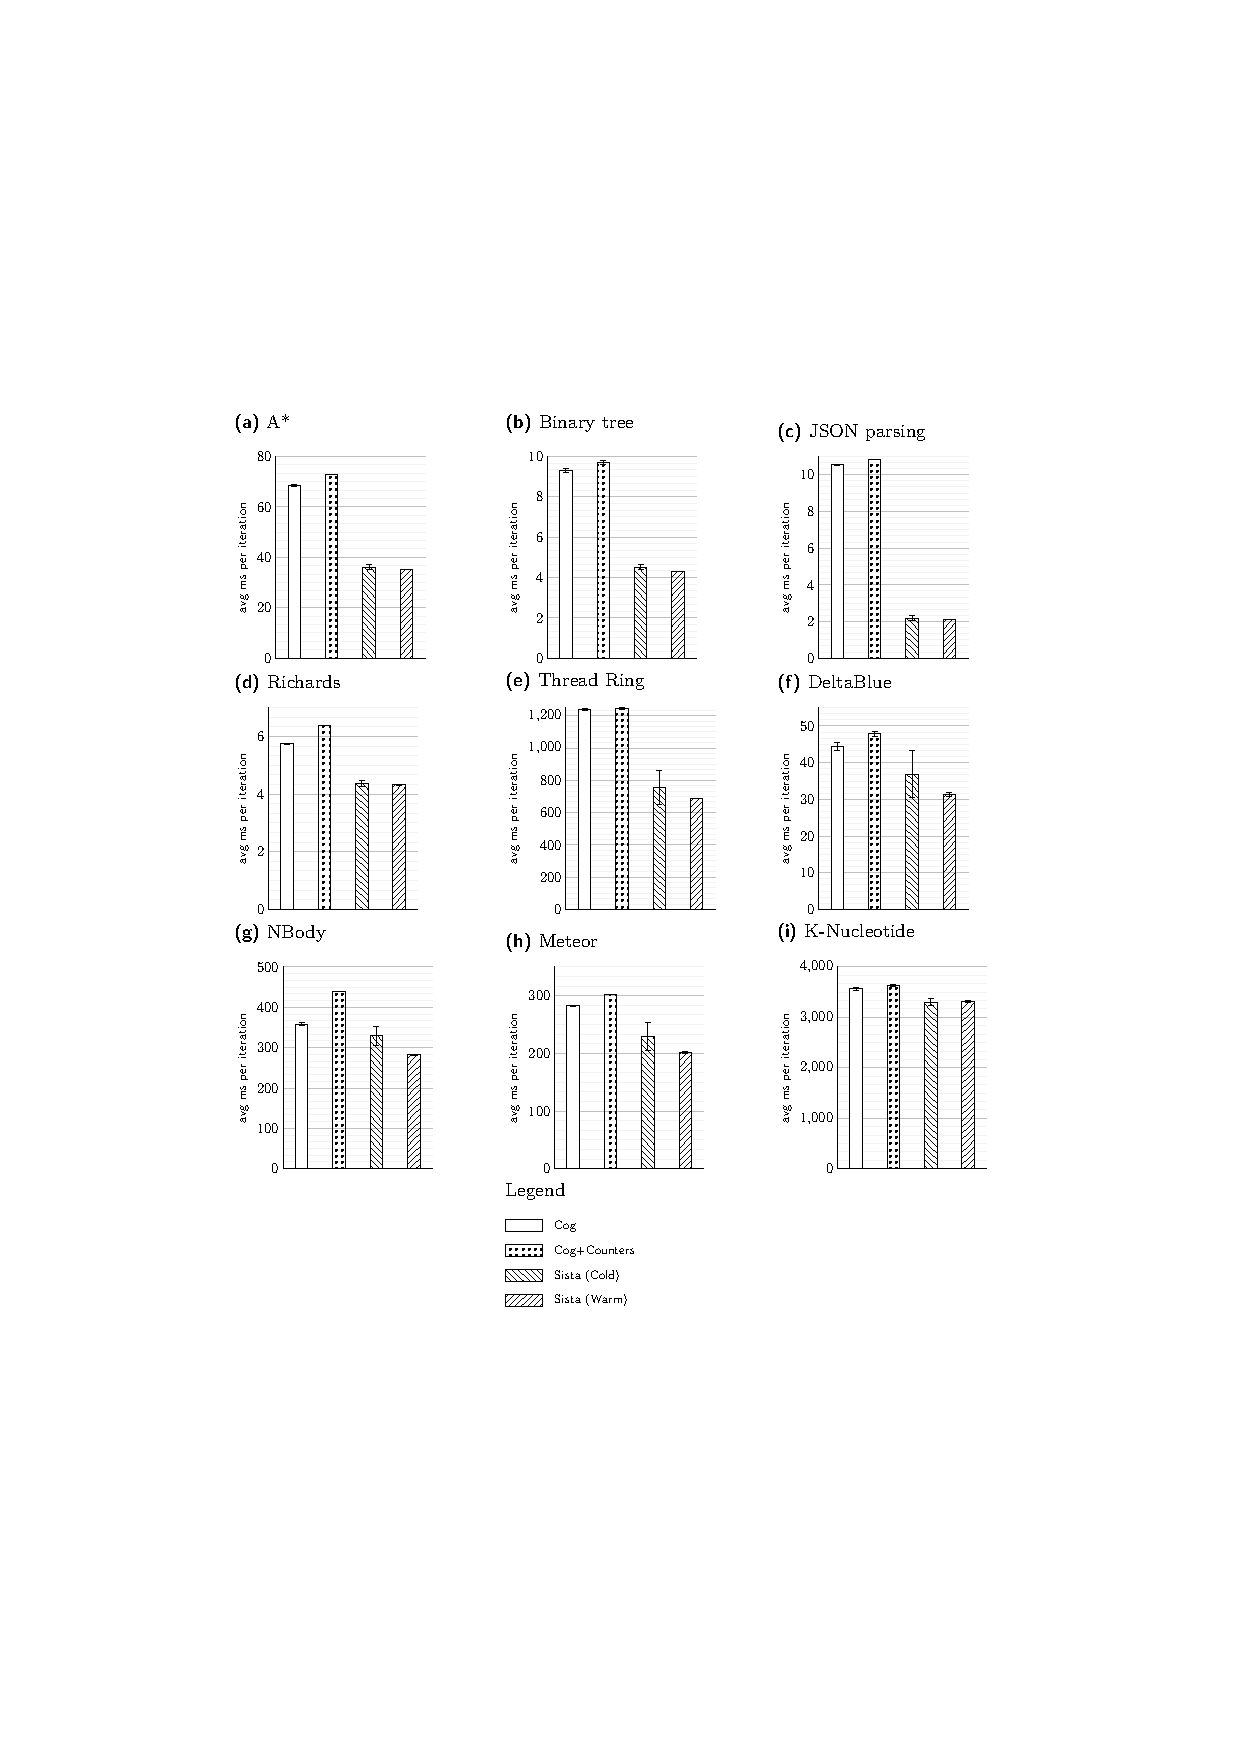
\includegraphics[width=\linewidth]{Bench}
        \caption{Benchmark measurements}
        \label{fig:measure}
    \end{center}
\end{figure}

\begin{figure}[h!]
    \begin{center}
        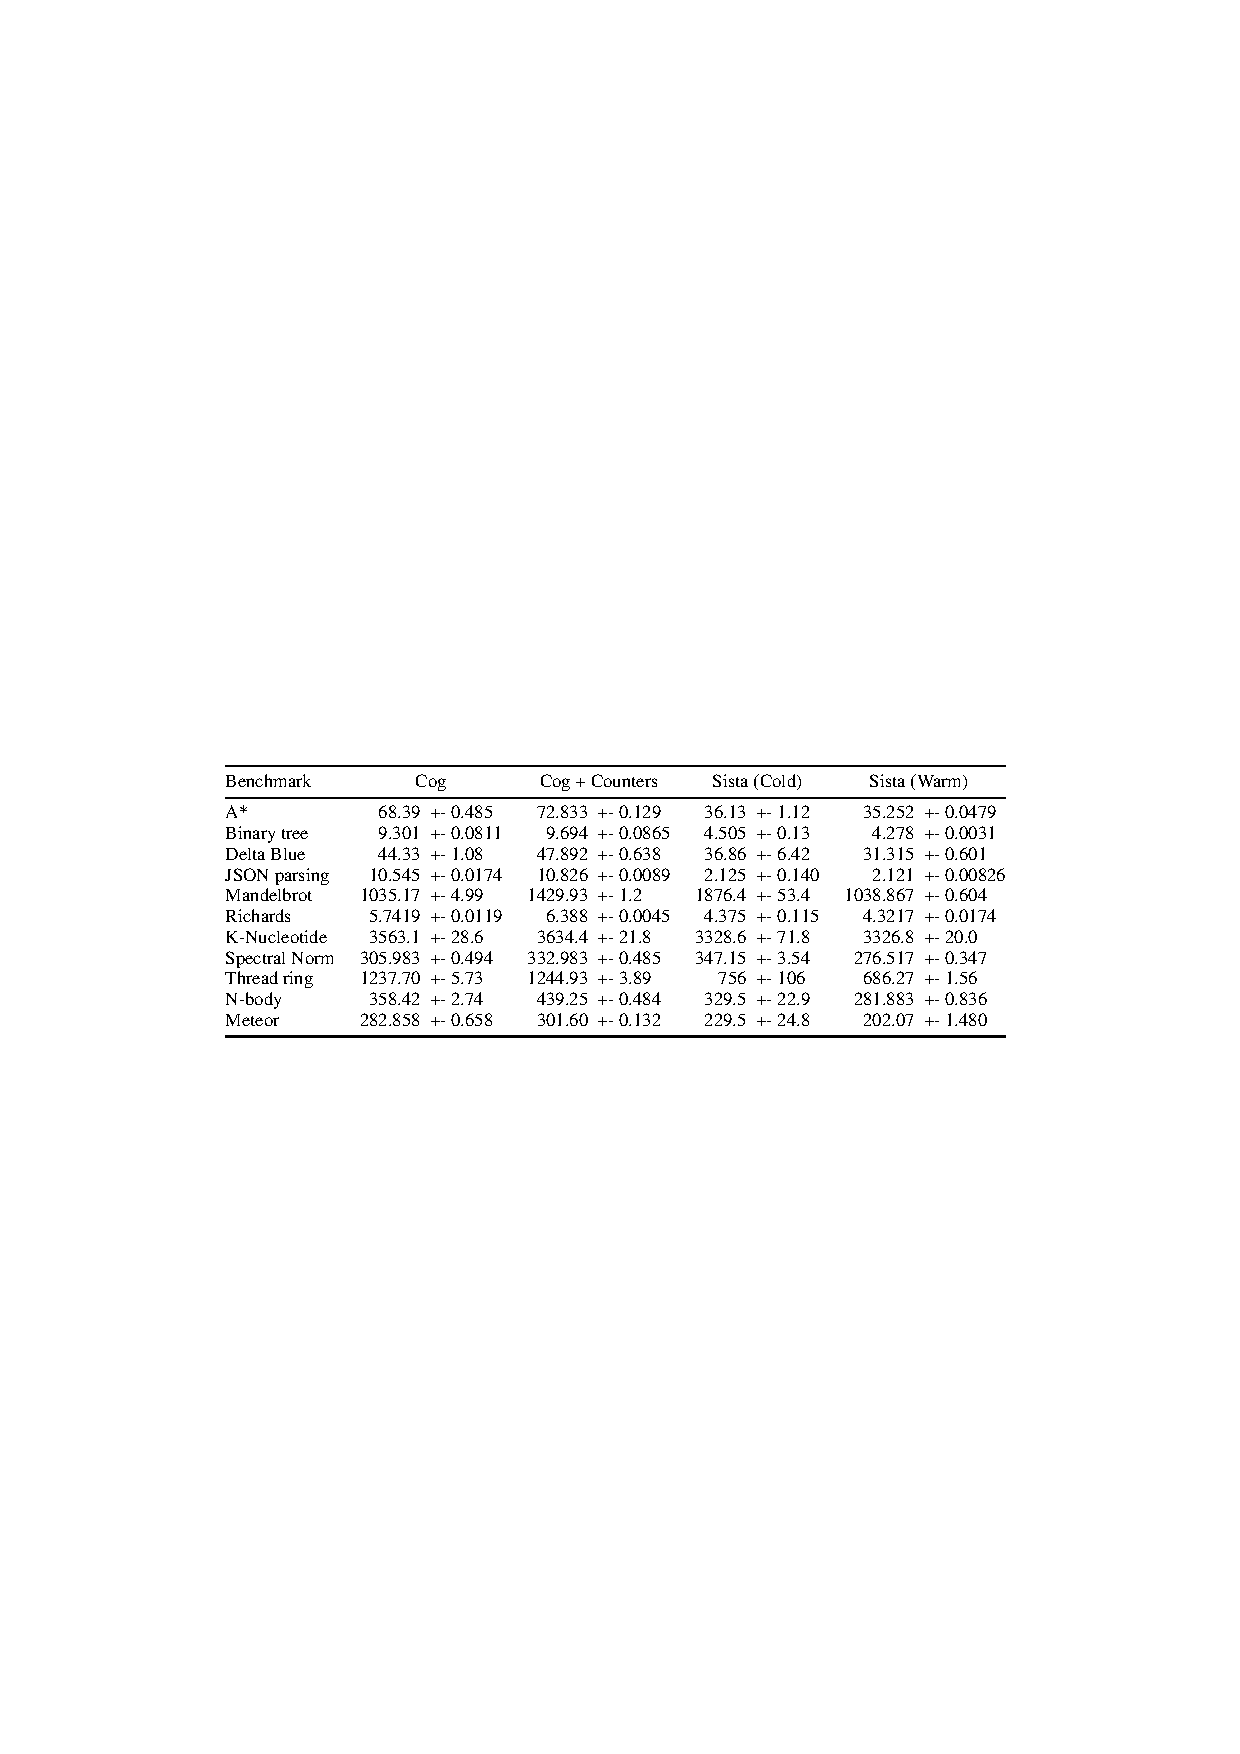
\includegraphics[width=\linewidth]{BenchTable}
        \caption{Benchmark results (standard errors in avg ms, 90\% confidence interval)}
        \label{tbl:benchmark}
    \end{center}
\end{figure}

\subparagraph{A*.}

The A* benchmark is a good approximation for applications where many objects collaborate. It measures parsing of large strings that define the layout of the nodes, message sending between each node, arithmetic to calculate costs, and collection operations. In the benchmark, we alternately parse and traverse two different graphs with 2,500 and 10,000 nodes, respectively. It is also a good benchmark for inlining block closures that are used in iterations.

Figure~\ref{fig:measure}(a) shows that adding counters to the VM comes with a slight overhead. A cold start for the benchmarks manages to improve the performance, with slight overhead due to the ongoing optimisations. Measuring the warmed up image, we see a significant improvement being about 50\% faster.                          

\subparagraph{Binary tree.}

The binary tree benchmark allocates, walks and deallocates binary trees. The benchmark is parameterized with  the maximum tree depth, which we have set to 10.

In this benchmark, peak performance of Sista is about 50\% faster than the standard VM, with very little error (Figure~\ref{fig:measure}(b)). The overhead of optimisation during a cold start leaves it around 5\% behind warm start.

\subparagraph{JSON parsing.}

We test a JSON parser written in Smalltalk as it parses a constant, minified, well-formed JSON string of 25 Kilobytes. This benchmark is heavy on nested loops and string operations, as well as a lot of parsing rules that call each other.

We can see a peak-performance is about 5 times faster (Figure~\ref{fig:measure}(c)). From a cold start, Sista improves performance with a bigger error margin due to the on-going optimisations.

\subparagraph{Richards.}

Richards is an OS kernel simulation benchmark that focuses on message sending between objects and block invocation. We ran this benchmark with the customary idle task, two devices, two handler tasks, and a worker, and filled the work queue of the latter three.

Figure \ref{fig:measure}(d) again shows a clear decrease in performance after adding counters to the VM. In this benchmark, the top-level benchmarking method is optimised very quickly, and only six optimised methods are installed in total. There is again no significant difference between the cold start Sista and the warmed up image. Both cases are a little over 25\% faster than the Cog VM without counters.

\subparagraph{Thread Ring benchmark.}

The Thread ring benchmark switches from thread to thread (green threads) passing one token between threads. Each iteration, 503 green threads are created and the token is passed around 5,000,000 times.

From an unoptimised snapshot, the first iteration of this benchmark is bound to be slow with our architecture, because multiple threads exist with the same code on the stack, each asking the profiler to optimise the same methods, while the optimiser refuses to do so because an optimised function already exists for the frequently used code. This induces a large error (Figure~\ref{fig:measure}(e)). Started again after warm-up, the optimised code runs over 40\% faster than the standard VM.

\subparagraph{DeltaBlue.}

DeltaBlue is a constraint solver, it tests polymorphic message sending and graph traversal. Each iteration tests updating a chain of 5000 connected variables once with equality constraints and once with a simple arithmetic scale constraint.

In this case, the benchmark takes a while to warm-up as many functions are inlined to allow optimisations to be performed (Figure~\ref{fig:measure}(f)). From a cold start, a large error is present due to the on-going optimisations. Started again after warm-up, the benchmark is 30\% faster than the standard VM.

\subparagraph{NBody.}

NBody models the orbits of Jovian planets, using a simple symplectic-integrator. At each iteration, the gravity interaction between each planets is computed to determine the next position of the planet.

NBody is a fairly large benchmark, taking enough time to warm-up to be seen from a cold start (Figure~\ref{fig:measure}(g)). Started after warm-up, the benchmark is 20\% faster than the standard VM.

\subparagraph{Meteor.}

Meteor is a puzzle-solver. Meteor takes a significant amount of time to warm-up, leading to a large error magin and sub-optimal performance when started on a cold VM (Figure~\ref{fig:measure}(h)). From a warmed-up snapshot, the benchmark is 30\% faster than the standard VM.

\subparagraph{k-Nucleotide.}

This benchmark reads a 2.4 MB DNA sequence string and counts all occurrences of nucleotides of lengths 1 and 2, as well as a number of specific sequences. It is a benchmark meant to test the performance of dictionaries in different languages, but serves well to test our inlining of small methods into loops.

The benchmark runs much slower than the others due to the large input, taking over 4 minutes to complete. Sista manages to optimise it to be about 10\% faster, with the cold start showing that the optimisation takes a while to amortize (Figure~\ref{fig:measure}(i)).

\subparagraph{Comments.}

We ran our VM profiler to profile the VM C code, but as for real world application, the time spent in the baseline JIT compiler generating machine code from bytecode is less than 1\% of the total execution time. As the runtime switches from interpreted code to machine code at second invocation for most functions and at first invocation for optimised functions, the time lost here is too small to be shown on our graphics. In fact, the time lost here is not significant compared to the variation so it is difficult to evaluate in our current setting. We believe that using a back-end doing many more machine low-level optimisations would increase the machine code compilation time and in this case we would be able to see a difference between the first run of pre-heated snapshot and second run as the VM still needs to produce the machine code for the optimised bytecoded functions.

Our optimiser is controlled by a number of variables that have been heuristically chosen to give good performance in a variety of cases. These include, among others, global settings for inlining depth, the allowed maximum size of optimised methods as well as methods to be inlined, as well as the time allowed for the optimiser to create an optimised method before it is aborted. We are working on fine-tuning these default values, as well as enabling heuristics to dynamically adapt these values depending on the application.

\section{Other validations}
\label{sec:otherValid}

To evaluate our infrastructure, we tried two other innovative techniques in addition to measuring benchmarks. On the one hand, we built an experimental technique to validate runtime deoptimisation using partial evaluation. On the other hand, we built a type inferencer using the runtime information extracted from inline caches. The promising results of the type inferencer confirm that the runtime information is quite precise and should give Scorch valuable hints to direct compiler optimisations.

\subsection{Experimental validation of the deoptimiser}

The speculative optimisations in the Sista VM enable many performance optimisations. However, they also introduce significant complexity. The compiler optimisations themselves, as well as the deoptimisation mechanism are complex and error prone. To stabilize Scorch, we designed a new approach to validate the correctness of dynamic deoptimisation. The approach~\cite{Bera16a} consists of the symbolic execution of an optimised and a non optimised v-function side by side, deoptimising the abstract stack at each point where dynamic deoptimisation is possible and comparing the deoptimised and non optimised abstract stack to detect bugs. 

Although this approach is interesting, the complexity required to maintain a good symbolic executor is significant compared to the time available for the maintenance of the overall VM. In other VMs such as V8~\cite{V8}, dynamic deoptimisation is stabilised using a "deopt-every-n-time" approach: the program run is forced to deoptimise the stack regularly (every n deoptimisation point met). This approach is way simpler to maintain and finds in practice a similar number of bugs than the approach built. We are now using a "deopt-every-n-time" approach to validate the deoptimisation of functions.

\subsection{Assessment of the runtime information quality}

Thanks to a new primitive method, any Pharo program, including Scorch, may request Cogit to provide the runtime information of a specific function. This runtime information is composed of the types met and functions called at each virtual call and the profiling counter values. To assess the quality of the runtime information provided for each virtual call, we built an approach called \emph{inline-cache type inference} (ICTI) to augment the precision of fast and simple type inference algorithms~\cite{Milo16a}. 

ICTI uses type information available in the inline caches during multiple software runs, to provide a ranked-list of possible classes that most likely represent a variable's type. We evaluated ICTI through a proof-of-concept that we implemented in Pharo Smalltalk. Analyzing the top-$n$+2 inferred types (where $n$ is the number of recorded runtime types for a variable) for 5486 variables from four different software systems (Glamour~\cite{Bung09a}, Roassal2~\cite{Pena13a}, Morphic~\cite{Fern07y} and Moose~\cite{Girb10a, Duca05a, Duca00b}) show that ICTI produces promising results for about 75\% of the variables. For more than 90\% of variables, the correct runtime type was present among first ten inferred types. Our ordering shows a twofold improvement when compared with the unordered base approach, \ie for a significant number of variables for which the base approach offered ambiguous results, ICTI was able to promote the correct type to the top of the list.

Based on this results, we believe the runtime information extracted from the first runs to be quite reliable. In any case, this information is used only to direct compiler optimisation: if the runtime information is not correct, the code is executed slower but correctly.

%%%%%%%%%%%%%%%%%%%%%%%%%%%%%%%%%%%%%%%%%%%%%%%%%%%%%%%%%%%%%%%%%%%%%%%%%%%%%%%%%%%%%%%%%%%%%%%%%%%%%%%%%%%%%%%%%%%%%%%%%%%%%%%%%%%%%%%%%%%%%%%%%%%

\section*{Conclusion}

This chapter validates Sista by showing on a range of benchmarks the performance gain of the architecture. The next Chapter discusses the future works that could be considered based on this thesis.

\ifx\wholebook\relax\else
    \end{document}
\fi